
\begin{multicols}{2}
    \begin{figure}[!htb]
        \centering
        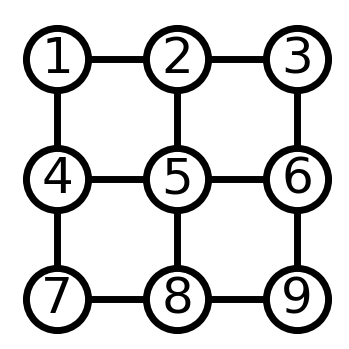
\includegraphics[width = 2.5cm]{graph_tri_equal}
        \caption{\label{fig: Graphe G}Graphe G}
    \end{figure}
    \begin{figure}[!htb]
        \centering
        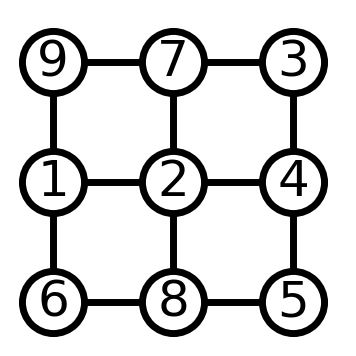
\includegraphics[width = 2.5cm]{cmg}
        \caption{\label{fig: Isomorphe G} Graphe $C_M(G)$}
    \end{figure}
\end{multicols}
    
\subsection{Application}

\begin{multicols}{2}
    \begin{figure}[!htb]
        \centering
        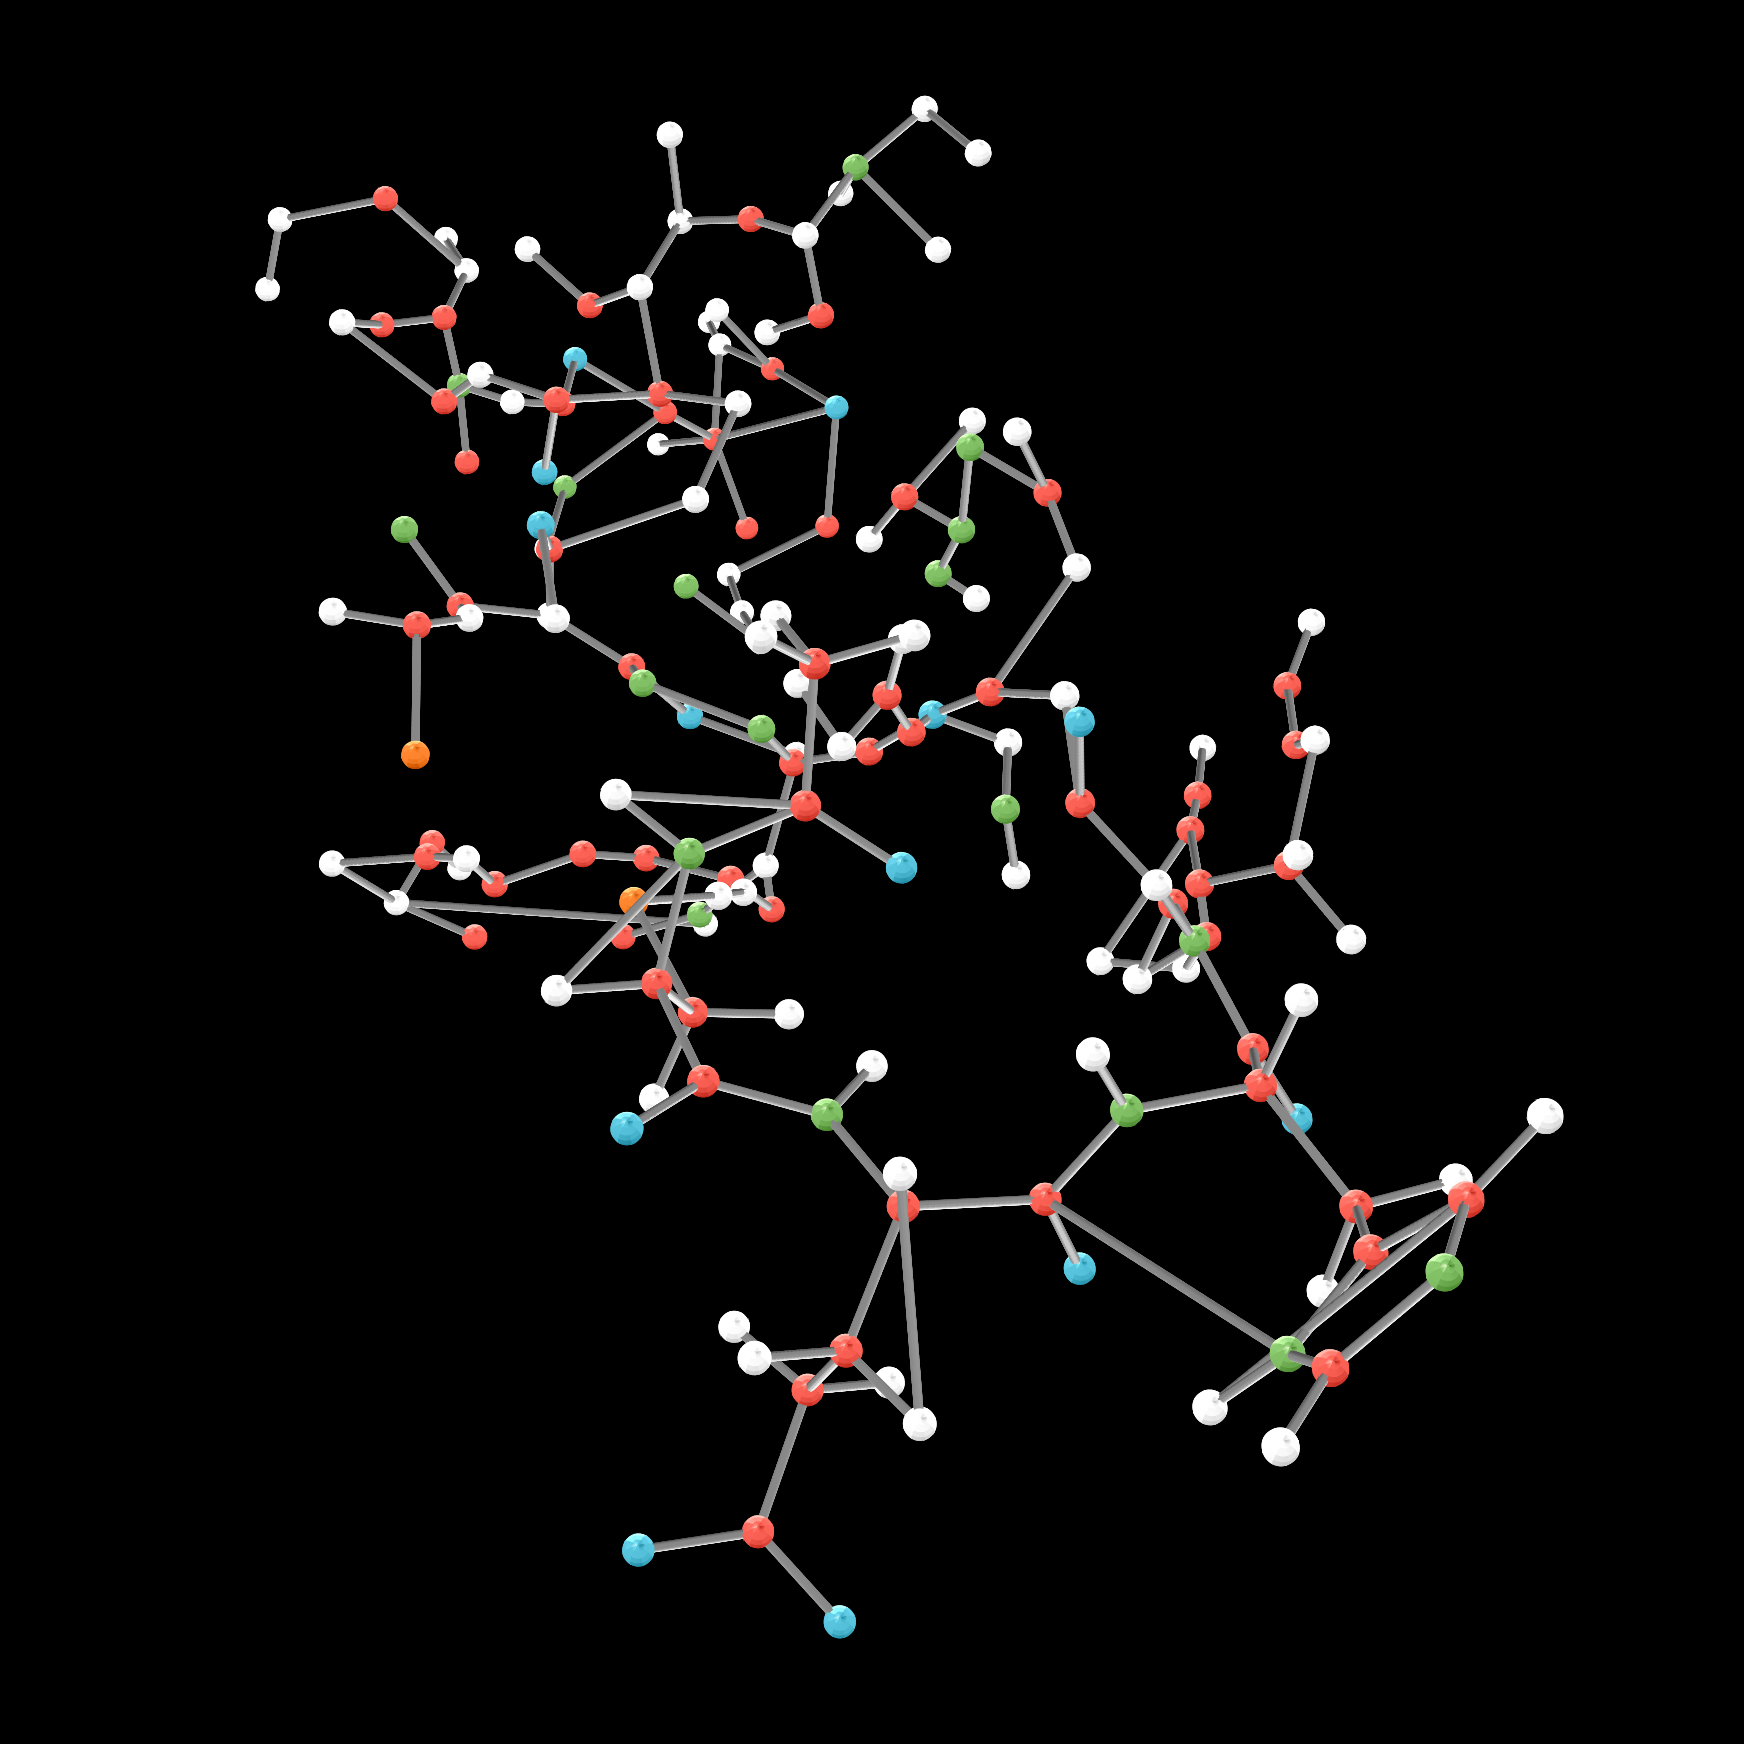
\includegraphics[width = 3cm]{protein_cov}
        \caption{\label{fig: Protéine}Protéine}
    \end{figure}
    \begin{center}
    \begin{figure}[!htb]
        \centering
        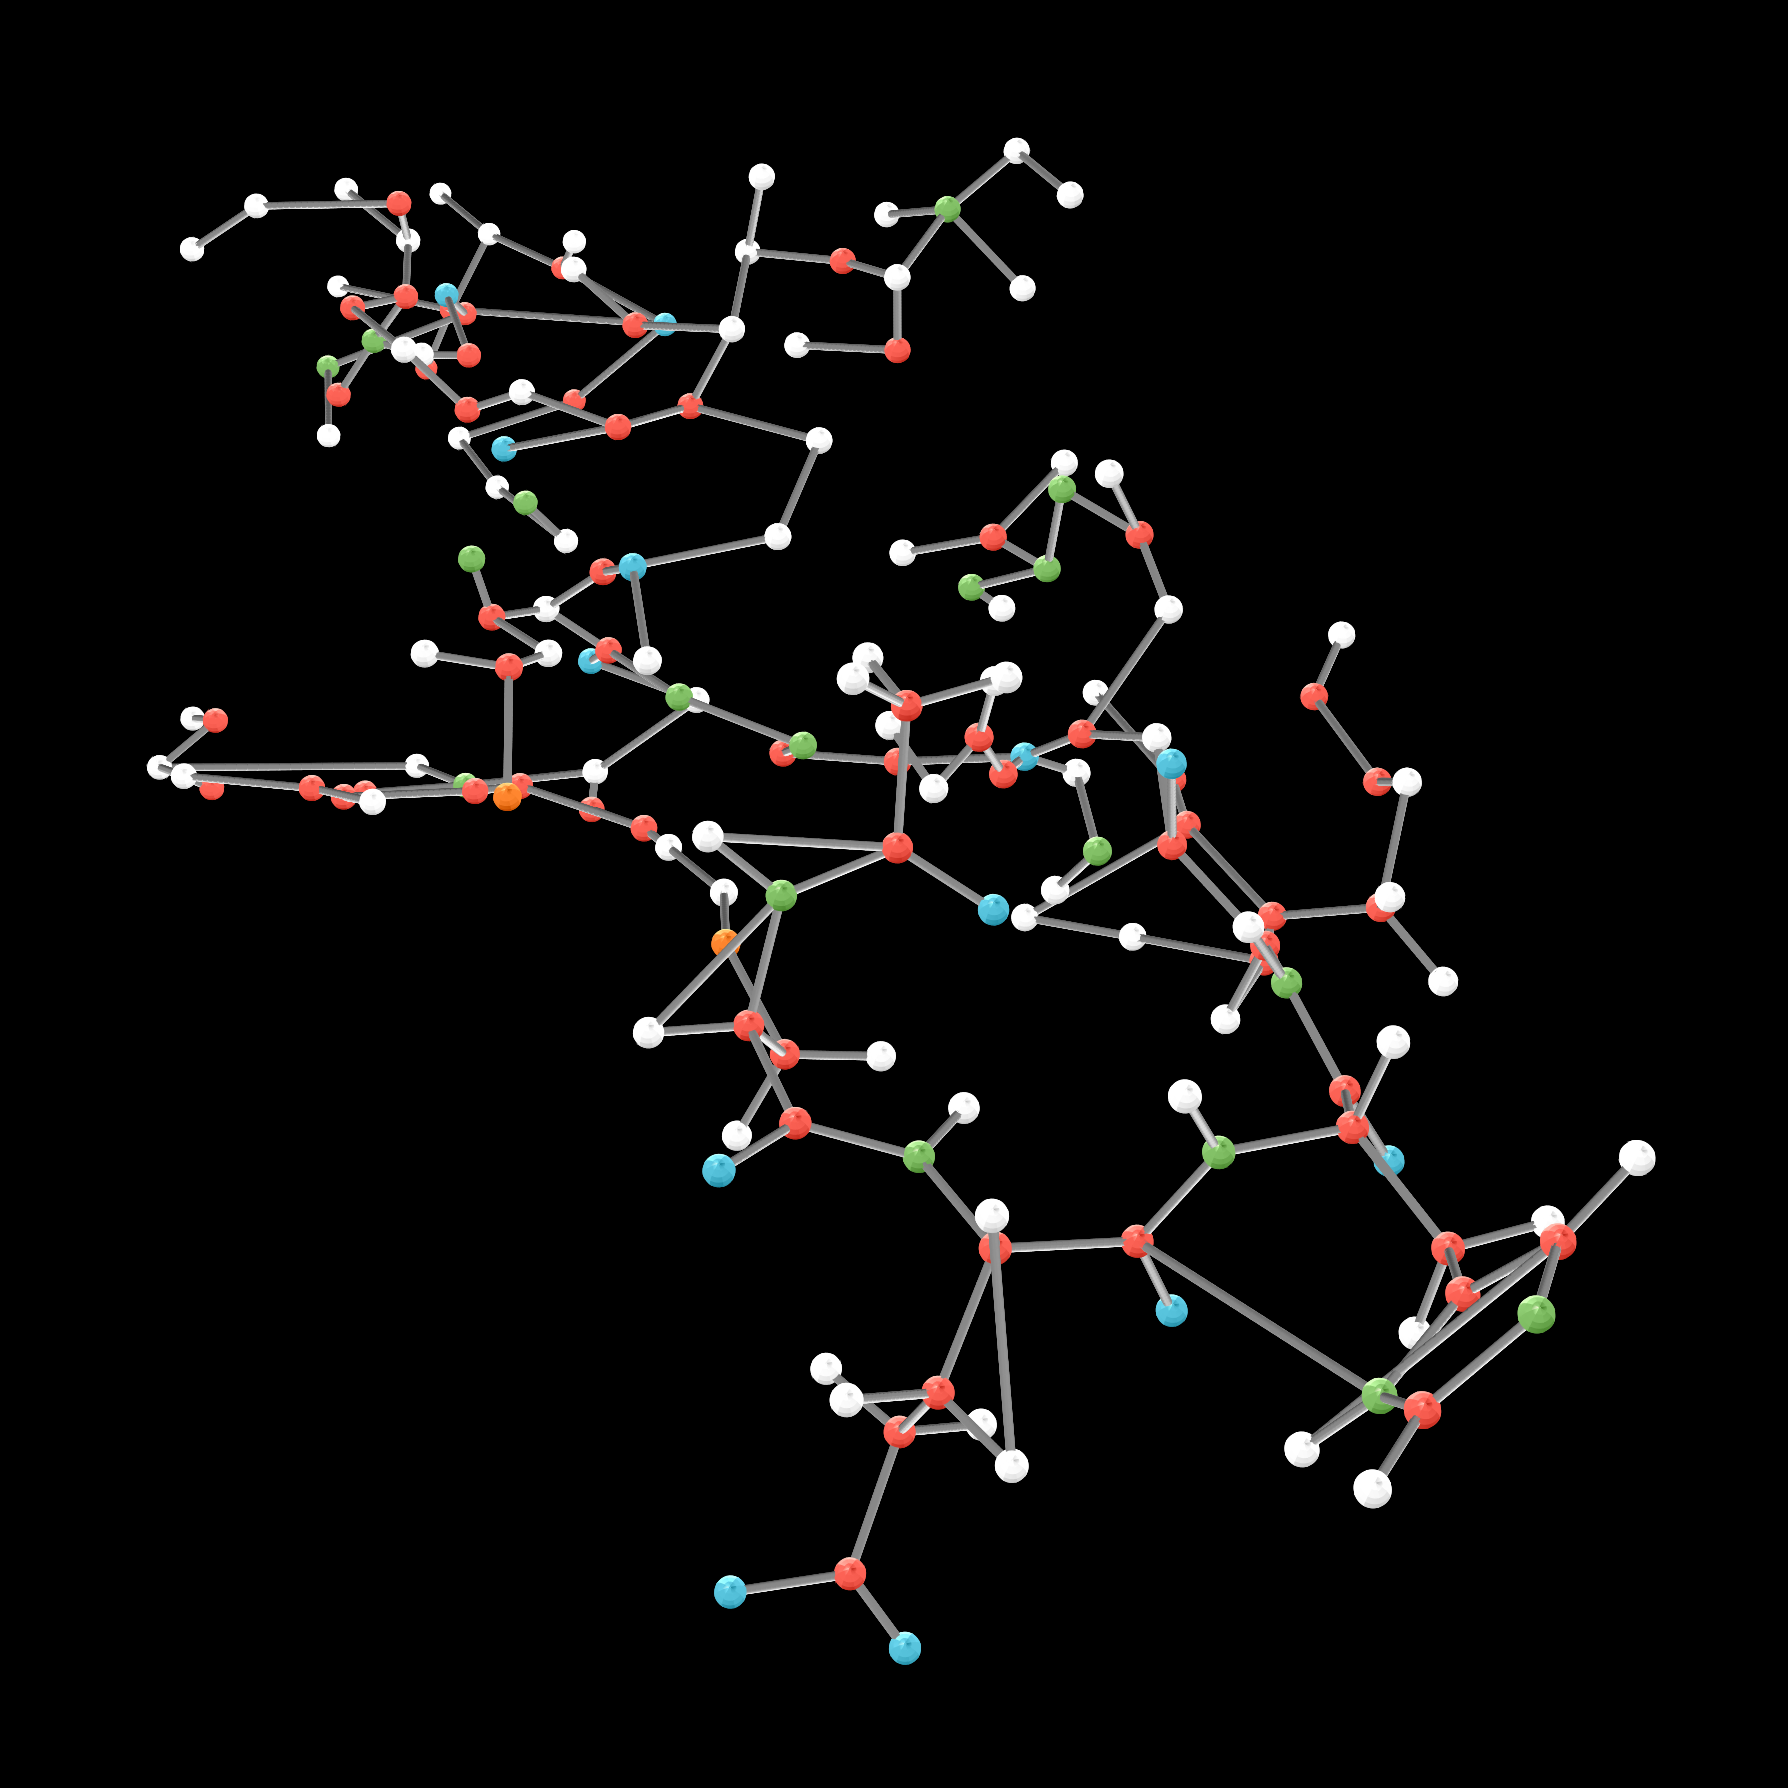
\includegraphics[width = 3cm]{protein_cov_translatee}
        \caption{\label{fig: Protéine translatée}Même protéine mais déplacée et numérotation différente des sommets}
    \end{figure}
    \end{center}
\end{multicols}
\underline{Temps d'éxecution} : pour cette protéine de 171 atomes
\begin{center}
\begin{tabular}{c|c}
    tri par degré et atomes & 0.002 s\\
    propagation des degrés & 7.4 s \\
    test d'isomorphisme & 0.3 s \\
    temps total d'éxecution & 7.8 s
\end{tabular}
\end{center}
\underline{Résultat} : protéines isomorphes et permutation renvoyée correcte
\newline tri + propagation du degré $\rightarrow$ paquets d'au plus 4 atomes
